%\documentclass[mathserif]{beamer}
\documentclass[handout]{beamer}
%\usetheme{Goettingen}
\usetheme{Warsaw}
%\usetheme{Singapore}
%\usetheme{Frankfurt}
%\usetheme{Copenhagen}
%\usetheme{Szeged}
%\usetheme{Montpellier}
%\usetheme{CambridgeUS}
%\usecolortheme{}
%\setbeamercovered{transparent}
\usepackage[english, activeacute]{babel}
\usepackage[utf8]{inputenc}
\usepackage{amsmath, amssymb}
\usepackage{dsfont}
\usepackage{graphics}
\usepackage{cases}
\usepackage{graphicx}
\usepackage{pgf}
\usepackage{epsfig}
\usepackage{amssymb}
\usepackage{multirow}	
\usepackage{amstext}
\usepackage[ruled,vlined,lined]{algorithm2e}
\usepackage{amsmath}
\usepackage{epic}
\usepackage{epsfig}
\usepackage{fontenc}
\usepackage{framed,color}
\usepackage{palatino, url, multicol}
\usepackage{listings}
%\algsetup{indent=2em}


\vspace{-0.5cm}
\title{Bayesian Linear Regression}
\vspace{-0.5cm}
\author[Felipe Bravo Márquez]{\footnotesize
%\author{\footnotesize  
 \textcolor[rgb]{0.00,0.00,1.00}{Felipe José Bravo Márquez}} 
\date{ \today }




\begin{document}
\begin{frame}
\titlepage


\end{frame}


%%%%%%%%%%%%%%%%%%%%%%%%%%%


\begin{frame}{Bayesian Linear Regression}
\scriptsize{
\begin{itemize}
\item In this class, which  is mostly based on chapter 4 of \cite{mcelreath2020statistical}, we are going to revisit the linear regression model from a Bayesian point of view.


\item The idea is the same: to model the relationship of a numerical dependent variable $\mathbf{y}$ with $n$ independent variables  $\mathbf{x}_1, \mathbf{x}_2, \dots, \mathbf{x}_n$ from a dataset $d$.

\item The response vaiable $\mathbf{y}$ is again modeled with a Gaussian distribution: $y_i \sim N(\mu_i,\sigma^2)$.


\item We also mantain the assumption that each attribute has a linear relationship to the mean of the outcome.

\begin{displaymath}
\mu_i = \beta_0 + \beta_1 x_i + \dots \beta_n x_n
\end{displaymath}

\item However, we are not going to use least squares or maximum likelihood to obtain point estimates of the parameters.

\item Instead, we are going to estimate the joint posterior distribution of all the parameters of the model:

\begin{displaymath}
f(\theta|d)= f(\beta_0,\beta_1,\dots,\beta_n,\sigma|d)
\end{displaymath}







 
\end{itemize}



} 

\end{frame}



\begin{frame}{Bayesian Linear Models}
\scriptsize{
\begin{itemize}


\item The Bayesian linear regresion is  more flexible than least squares as it allows incorporating prior information.

\item It also allows to interpret the uncertainty of the model in a clearer way.

\item Notice that the the parameters of the model are $\beta_0,\beta_1,\dots,\beta_b$ and $\sigma$ but not $\mu_i$.

\item This is because $\mu_i$ it is determined deterministically from the linear model's coefficients.

\item In order to build our posterior we need to define a likelihood function:

\begin{displaymath}
 f(d|\beta_0,\beta_1,\cdots,\beta_n,\sigma) =\prod_{i=1}^m f(d_i|\beta_0,\beta_1,\cdots,\beta_n,\sigma) 
\end{displaymath}


\item Where $d_i$ corresponds to each data point in the dataset containing values for $y$ and $x_1,\dots,x_n$ (IID assumption).

\item The likelihood of each point is modeled with a Gaussian distribution:

\begin{displaymath}
 f(d_i|\beta_0,\beta_1,\cdots,\beta_n,\sigma)= N(\mu_i, \sigma^2)
\end{displaymath}



 
\end{itemize}



} 

\end{frame}



\begin{frame}{Bayesian Linear Models}
\scriptsize{
\begin{itemize}


\item Now we need a joint prior density:

\begin{displaymath}
f(\theta)= f(\beta_0,\beta_1,\dots,\beta_n,\sigma)
\end{displaymath}


\item And the posterior gets specified as follows:

\begin{displaymath}
f(\theta|d)= \frac{ \prod_{i=1}^m f(d_i|\beta_0,\beta_1,\cdots,\beta_n,\sigma)*f(\beta_0,\beta_1,\dots,\beta_n,\sigma)}{f(d)}
\end{displaymath}


\item The evidence is expressed by a multiple integral:

\begin{displaymath}
 f(d) = \int \int \dots \int \prod_{i=1}^m f(d_i|\beta_0,\beta_1,\cdots,\beta_n,\sigma)* f(\beta_0,\beta_1,\dots,\beta_n,\sigma) d\beta_0 d\beta_1 \cdots d\beta_nd\sigma
\end{displaymath}



\item In most cases, the priors are specified independently for each parameter, which is equivalent to assuming:


\begin{displaymath}
f(\beta_0,\beta_1,\cdots,\beta_b,\sigma)=f(\beta_0)*f(\beta_1)*\dots*f(\beta_n)*f(\sigma). 
\end{displaymath}






 
\end{itemize}



} 

\end{frame}



\begin{frame}{A model of height revisited}
\scriptsize{
\begin{itemize}
 \item   To understand this more concretely, we will rebuild the linear model relating the height and weight of the !Kung San people using a Bayesian approach.
 
 \item We will refer to each person's height and weight as $y_i$ and $x_i$ respectively.
 
 \item Our probabilistic model specifying all components of a Bayesian model is defined as follows:
 
 \vspace{0.3cm}
 \begin{table}
 \centering
 \begin{tabular}{lr}  
$y_i \sim N(\mu_i,\sigma)$ & [likelihood] \\
$\mu_i = \beta_0 + \beta_1 x_i$ & [linear model] \\
$\beta_0 \sim N(150,50)$ & [$\beta_0$ prior] \\
$\beta_1 \sim N(0,1)$ & [$\beta_1$ prior] \\
$\sigma \sim $ Uniform$(0,50)$ & [$\sigma$ prior] \\
\end{tabular}
\end{table}

 \vspace{0.3cm}

 \item   Parameters $\beta_0$ and $\beta_1$ are the intercept and the slope of our linear model.
 
 \item The parameter $\sigma$ is the standard deviation of all the heights.
 
 \item Note that we are setting the same $\sigma$ for all observations, which is equivalent to the Homoscedasticity property of the standard linear regression. 
 


 
\end{itemize}
 

 
}
\end{frame}


\begin{frame}{A model of height revisited}
\scriptsize{
\begin{itemize}
 
  \item  Our priors were set independently for each parameter which implies that the joint prior density $f(\beta_0,\beta_1,\sigma)$ can be expressed as $f(\beta_0)*f(\beta_1)*f(\sigma)$.
 
 \item It should be kept in mind that the choice of priors is subjective and should be evaluated accordingly.
 
 \item Let's try to justify our choice a bit:
 
 \begin{enumerate}
 \scriptsize{
  \item The Gaussian prior for $\beta_0$ (intercept), centered on 150cm with a standard variation of 50, covers a huge range of plausible mean heights for human populations while giving very little chance for negative heights. \vspace{0.2cm}
  \item The Gaussian prior for $\beta_1$ (slope), centered on 0 with a standard variation of 1, acts as a \textbf{regularizer} to prevent the model from \textbf{overfitting} the data by assigning extreme values to $\beta_1$.\footnote{Regularization and overfitting will be discussed later in the course.}  \vspace{0.2cm} 
    \item The uniform prior for the standard deviation $\sigma$ between 0 and 50 prohibits obtaining negative standard deviations. The upper bound (50 cm) would imply that 95\% of individual heights lie within 100cm of the average height. That's a very large range.  \vspace{0.2cm}
}
 \end{enumerate}

  

 
\end{itemize}
 

 
}
\end{frame}


\begin{frame}[fragile]{Fitting the Model}
\scriptsize{
\begin{itemize}
 
  \item Now we need to fit the model to the data to build the posterior distribution.
  
  \item Grid approximation is not a valid option, as setting up a grid for 3 parameters would be too computationally expensive.
  
  \item We will use Laplace approximation instead.
  
  \item In this approach we obtain the MAP estimates for each parameter using a hill-climbing \textbf{optimization} method.
  
  \item Then we fit a \textbf{multivariate Gaussian distribution} centered on these values.
  
  
  \item This distribution is the multidimensional extension to the standard Gaussian.
  

 
\end{itemize}
 

 
}
\end{frame}

\begin{frame}[fragile]{The multivariate Gaussian distribution}
\scriptsize{
\begin{itemize}
 
  \item The multivariate Gaussian distribution in $d$-dimensions defined by the following density function (PDF):
  
  \begin{displaymath}
   f_x = \frac{1}{(2\pi)^{d/2}|\Sigma|^{1/2}}\exp \left( -\frac{1}{2}(\vec{x}-\vec{\mu})^T  \Sigma^{-1}(\vec{x}-\mu)\right)
  \end{displaymath}

  
\item This density function allows working with a $d$-dimensional vector of random variables $\vec{X}$.


\item The first parameter of this distributions is a mean vector $\vec{\mu} \in \mathcal{R}^d$ with the mean value of each dimension.

\item The second parameter is a covariance matrix $\Sigma \in R^{d\times d}$,

\item This matrix contains the variance of each variable in the diagonal and the covariance of variables $X_i$ and $X_j$ in the other cells $\Sigma_{i,j}$:

\begin{displaymath}
 Cov(X) = \Sigma
\end{displaymath}

\item The matrix $\Sigma$ is symmetric and positive semi-definite.
  
\item The multivariate Gaussian $N(\vec{\mu},\Sigma)$ is a very convenient distribution for modeling multidimensional random variables.
  
  
 
\end{itemize}
 

 
}
\end{frame}



\begin{frame}[fragile]{The multivariate Gaussian distribution}
\scriptsize{
\begin{itemize}
 
  \item Here are some examples taken from \cite{ng2008generative} of what the density of a multivariate Gaussian distribution looks like:
  
  \begin{figure}[h!]
	\centering
	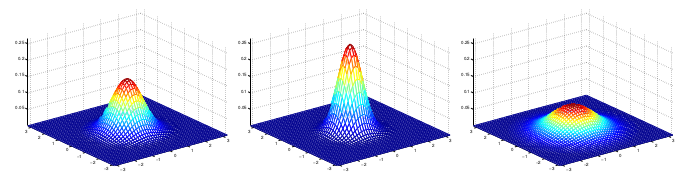
\includegraphics[scale=0.4]{pics/mgaussian1.png}
\end{figure}


\item The left-most figure shows a Gaussian with mean zero (that is, the 2x1 zero-vector) and covariance matrix $\Sigma = I$ (the $2\times2$ identity matrix). 
\item A Gaussian with zero mean and identity covariance is also called the standard normal distribution.

\item The middle figure shows the density of a Gaussian with zero mean and $\Sigma = 0.6I$.

\item The rightmost figure shows one with , $\Sigma = 2I$.

\item We see that as $\Sigma$ becomes larger, the Gaussian becomes more ``spread-out'', and as it becomes smaller, the distribution becomes more ``compressed''.
 
\end{itemize}
 

 
}
\end{frame}





\begin{frame}[fragile]{The multivariate Gaussian distribution}
\scriptsize{


  
  \begin{figure}[h!]
	\centering
	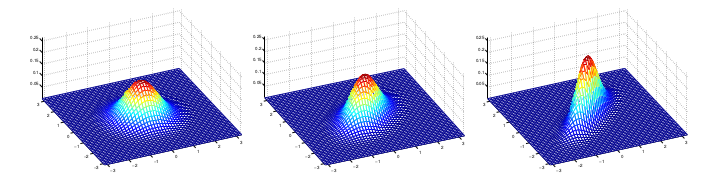
\includegraphics[scale=0.4]{pics/mgaussian2.png}
\end{figure}
 
\begin{itemize}
 

 \item The figures above show Gaussians with mean 0, and with covariance matrices respectively
 
   \begin{figure}[h!]
	\centering
	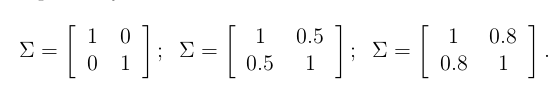
\includegraphics[scale=0.35]{pics/mgaussian4.png}
\end{figure}

\item The leftmost figure shows the familiar standard normal distribution, and we see that as we increase the off-diagonal entry in $\Sigma$, the density becomes more ``compressed'' towards the $45\cdot$ line (given by $x_1 = x_2$).
 
\end{itemize}
 

 
}
\end{frame}





\begin{frame}[fragile]{The multivariate Gaussian distribution}
\scriptsize{
\begin{itemize}
 
  \item   As our last set of examples, fixing $\Sigma = I$, by varying $\vec{\mu}$ we can also move the mean of the density around.
  
  \begin{figure}[h!]
	\centering
	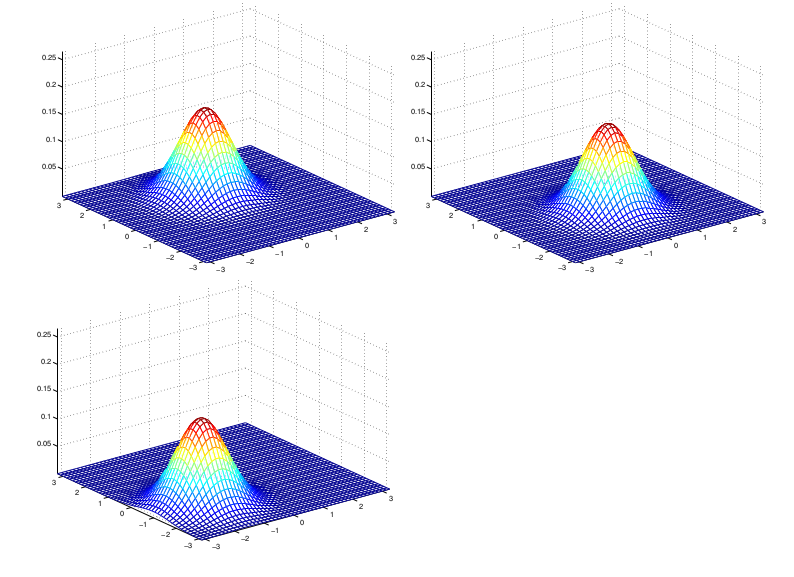
\includegraphics[scale=0.25]{pics/mgaussian3.png}
\end{figure}
 

 \item The figures above were generated using $\Sigma = I$, and respectively
 
   \begin{figure}[h!]
	\centering
	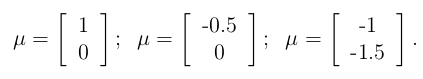
\includegraphics[scale=0.3]{pics/mgaussian5.png}
\end{figure}
 
\end{itemize}
 

 
}
\end{frame}


\begin{frame}{Laplace approximation}
\scriptsize{

\begin{itemize}
\item In Laplace approximation we assume that the joint posterior follows a multivariate Gaussian distribution $f(\theta_1,\dots,\theta_n) = N(\vec{\mu},\Sigma)$.

\item  According to \cite{gelman2013bayesian}, this approximation is convenient for unimodal and roughly symmetric posterior distributions.

\item There are also a theoretical asymptotic argument in favor of this approximation: ``if the dataset is large enough, a posterior distribution can be approximated by a Gaussian'' \cite{gelman2013bayesian}.

\item The values of $\vec{\mu}$ are obtained from the posterior mode of each parameter (MAP):
\begin{displaymath}
 \vec{\mu} = \vec{\theta}_{MAP}
\end{displaymath}

\item Which are obtained using numeric optimization techniques.


\end{itemize}


} 
\end{frame}



\begin{frame}{Laplace approximation}
\scriptsize{

\begin{itemize}

\item The values of $\Sigma$ are obtained from the curvature near these values, which are obtained from the second derivatives of the posterior:

\begin{displaymath}
 \Sigma = [I({\theta}_{MAP})]^{-1}
\end{displaymath}

where  \begin{displaymath}
        I(\theta) = - \frac{d^2}{d\theta^2} \log f(\theta|d)
       \end{displaymath}



\item Notice that both  $\vec{\mu}$ and $\Sigma$ can be calculated from the unnormalized posterior 
$f(d|\theta)*f(\theta)$

\item We don't need to calculate the evidence $f(d)$ to perform Laplace approximation \cite{laplaceApp}.

\end{itemize}


} 
\end{frame}


\begin{frame}[fragile]{Fitting the Model}
\scriptsize{
\begin{itemize}
 
  \item Laplace approximation is implemented in the \textbf{quap} function from the \textbf{rethinking} package.
  
  \item The model for height defined above can be implemented as follows:
  
  \begin{verbatim}
library(rethinking)
data(Howell1)
d <- Howell1
d2 <- d[ d$age >= 18 , ]

b.reg1 <- quap(
  alist(
    height ~ dnorm( b0 + b1*weight, sigma ),
    b0 ~ dnorm( 150 , 50 ) ,
    b1 ~ dnorm( 0 , 1) ,
    sigma ~ dunif( 0 , 50 )
  ) , data=d2 )
  \end{verbatim}

  

 
\end{itemize}
 

 
}
\end{frame}

\begin{frame}[fragile]{Fitting the Model}
\scriptsize{
\begin{itemize}
 
  \item We can summarize this posterior with the command \textbf{precis}:
  
  \begin{verbatim}
> precis( b.reg1, prob=0.95 )
        mean   sd   2.5%  97.5%
b0    113.99 1.90 110.26 117.71
b1      0.90 0.04   0.82   0.98
sigma   5.07 0.19   4.70   5.45
  \end{verbatim}

\item These numbers provide Gaussian approximations for each parameter's \textbf{marginal} posterior distribution.

\item A marginal is the distribution of a parameter $\theta_i$ regardless of the values of the others.


\item In mathematical terms this is obtained, after integrating (averaging) over  $\theta_j \ \forall j \neq i$:

\begin{displaymath}
f(\theta_i |d) = \int \dots \int f(\theta_1,\dots,\theta_n|d)d\theta_1,\dots,d\theta_{i-1},d\theta_{i+1},\dots,d\theta_{n} 
\end{displaymath}

 
\end{itemize}
 

 
}
\end{frame}


\begin{frame}[fragile]{Fitting the Model}
\scriptsize{
\begin{itemize}

\item We can compare the mean and standard deviation of $\beta_0$ and $\beta_1$ with what we obtained using least squares in previous lecture.

\begin{verbatim}
> summary(reg1)
...

Coefficients:
             Estimate Std. Error t value Pr(>|t|)    
(Intercept) 113.87939    1.91107   59.59   <2e-16 ***
weight        0.90503    0.04205   21.52   <2e-16 ***
---
Signif. codes:  0 ‘***’ 0.001 ‘**’ 0.01 ‘*’ 0.05 ‘.’ 0.1 ‘ ’ 1

Residual standard error: 5.086 on 350 degrees of freedom
....
\end{verbatim}


\item The values are almost the same!

\item Recall that maximum likelihood or least squares estimators are identical to MAP estimators with uniform priors.

\item This indicates that our priors did not have a significant impact.
 
\end{itemize}
 

 
}
\end{frame}

\begin{frame}[fragile]{Covariance Matrix}
\scriptsize{
\begin{itemize}

\item Because in Laplace Approximation we are using a multivariate Gaussiand we can also get the covariance matrix $\Sigma$.

\begin{verbatim}
> vcov( b.reg1 )
                b0            b1         sigma
b0     3.620141920 -7.884254e-02  1.765417e-03
b1    -0.078842537  1.752477e-03 -3.830179e-05
sigma  0.001765417 -3.830179e-05  3.654305e-02 
\end{verbatim}


\item The matrix tell us it tells how each parameter relates to every other parameter in the posterior distribution.

\item We can converte these covariances into correlation coefficients to facilitate its interpretability:

\begin{verbatim}
> cov2cor( vcov( b.reg1 ) )
                b0           b1        sigma
b0     1.000000000 -0.989855066  0.004853802
b1    -0.989855066  1.000000000 -0.004786196
sigma  0.004853802 -0.004786196  1.000000000
\end{verbatim}



\end{itemize}
 

 
}
\end{frame}


\begin{frame}{Conclusions}
\scriptsize{

\begin{itemize}
\item Blabla
\end{itemize}


} 
\end{frame}


%%%%%%%%%%%%%%%%%%%%%%%%%%%
\begin{frame}[allowframebreaks]\scriptsize
\frametitle{References}
\bibliography{bio}
\bibliographystyle{apalike}
%\bibliographystyle{flexbib}
\end{frame}  









%%%%%%%%%%%%%%%%%%%%%%%%%%%

\end{document}
